

\documentclass[a4paper,12pt]{article}
\usepackage{amsmath}
\usepackage{amsfonts}
\usepackage{amssymb}
\usepackage{graphicx}
\usepackage{isotope}
\newcounter{saveenumi}
\usepackage{tikz}
\usetikzlibrary{shapes.geometric}
\usetikzlibrary{decorations.pathmorphing}
\usetikzlibrary{trees}
\usetikzlibrary{decorations.pathmorphing}
\usetikzlibrary{decorations.markings}
\providecommand{\e}[1]{\ensuremath{\times 10^{#1}}}

% Define styles for the different kind of edges in a Feynman diagram
\tikzset{
    boson/.style={decorate, decoration={snake}, draw=black},
    photon/.style={decorate, decoration={snake}, draw=black},
    electron/.style={draw=black, postaction={decorate},
        decoration={markings,mark=at position .55 with {\arrow[draw=black]{latex}}}},
    gluon/.style={decorate, draw=black,
        decoration={coil,amplitude=4pt, segment length=5pt}} 
}

\addtolength{\voffset}{-2cm}
\addtolength{\textheight}{4cm}

\title{AQA Unit PHYA1: Particles, Radiation and Quantum Phenomena}
\author{\textsc{A.C. Norman}
\\ \texttt{anorman@bishopheber.cheshire.sch.uk}}
\date{August 27, 2011}

\begin{document}
\maketitle

%\part{Particles and Radiation}

\section{Constituents of the atom}

The table below summarizes the particles which make up matter\\

\begin{tabular}{lcccc}
\hline
Name & Location & Charge / C & Relative mass & Actual mass / kg\\
\hline
Proton & nucleus & +1.6\e{-19} & 1 & 1.67\e{-27}\\
Neutron & nucleus & 0 & 1 & 1.67\e{-27}\\
Electron & orbitals & $-1.6\e{-19}$ & $1/1833$ & 9.11\e{-31}\\
\hline
\end{tabular}\\

The atom comprises a tiny ($\approx 10^{-14}$~m) nucleus, containing protons and neutrons, around which are electrons in atomic orbitals (of radius $\approx 10^{-10}$~m).

An atom is written as\\

{\huge \isotope[{\it A}][{\it Z}]{X}}\\

where \begin{minipage}[t]{12cm}$A$ is the nucleon number (the number of protons and neutrons),\\
$Z$ is the proton number, and\\
X is the element symbol.\end{minipage}

\subsection{Proton number, $Z$}

Also called the atomic number.  This defines the element, and therefore dictates its properties.  In an atom, the number of electrons will equal the proton number; in an ion, there will be fewer of more electrons than $Z$.

\subsection{Nucleon number, $A$}

Also called the mass number.  This is the total number of nucleons (i.e.\ protons + neutrons) in the nucleus.

The number of neutrons is therefore $A-Z$.  All nuclei, except for one isotope of hydrogen, contain neutrons.  The neutrons hold together the protons, which electrostatically repel each other.

In general, for lower $Z$ elements, there are roughly the same numbers of protons and neutrons, but the number of neutrons increases more rapidly as large nuclei are made.

The number of neutrons have no effect on the chemical properties of the element, but may make it more or less stable and therefore determine whether an element is radioactive.

\subsection{Isotopes}

Isotopes are nuclides with the same proton number, but different nucleon numbers (i.e. same number of protons, but different numbers of neutrons).

Many elements exist in several stable isotopes, and they are not given separate names, except for:
\begin{itemize}
\item \isotope[1][1]{H} is hydrogen.
\item \isotope[2][1]{H} is deuterium.
\item \isotope[3][1]{H} is tritium.
\end{itemize}

%\section{Stable and unstable nuclei}

%[to be expanded]

\section{Particles, antiparticles and photons}

Every particle that exists has an antiparticle.  Antiparticles do not exist as constituents of ordinary matter, but are easily created in particle accelerators, and are produced in radioactive decay and cosmic rays.

For every particle:
\begin{itemize}
\item its antiparticle has the same mass
\item its antiparticle has equal but opposite charge (as well as other associated numbers)
\item an unstable particle has the same half-life as its antiparticle
\end{itemize}

\subsection{Stable particles}

The following particles are the only particles which are stable:\\

\begin{tabular}{lccc}
\hline
\hline
Name & Symbol & Charge ($Q$) / $e$ & Rest mass / kg \\
\hline
electron & e$^{-}$ & $-1$ & 9.1\e{-31} \\
positron & e$^{+}$ & $+1$ & 9.1\e{-31} \\
proton & p & $+1$ & 1.6\e{-27} \\
antiproton & $\bar{\mathrm{p}}$ & $+1$ & 1.6\e{-27} \\
neutrino & $\nu$ & $+1$ & $\sim 10^{-37}??$ \\
antineutrino & $\bar{\nu}$ & $+1$ & $\sim 10^{-37}??$ \\
\hline
\hline
\end{tabular}

\paragraph{Notes}\begin{enumerate}
\item The antiparticles are stable in isolation: in practice, they would encounter a particle and annihilate.
\item There are three kinds of neutrino, and therefore three antineutrinos (in fact, neutrinos are constantly shifting between these three flavours of neutrino -- this is how physicists know they have mass!)
\item Some particles are identical to their anti-particle, e.g. the photon, and the $\pi^{0}$ (pi-meson).
\item In general, particle symbols are made into their antiparticle by the `bar' above the symbol.
\end{enumerate}

\subsubsection{Neutrinos}

Neutrinos are the most common particles in the universe, outnumbering the number of protons by about a billion to one.  The are emitted in nuclear reactions such as those that occur inside the sun.

They are very difficult to detect, even though 6\e{10} pass through every square centimetre of the earth every second.  They interact very weakly, and this is why their mass was not discovered until recently, and is an area of ongoing research.

The neutrino was predicted to exist in 1930, and was postulated due to the range of energies of beta particles in radioactive beta decay.

\subsection{Annihilation}

When a particle meets its antiparticle, the particles annihilate.  They cease to exist, and in their place {\bf two} photons are created, of gamma ray energies.

The mass of the particles is converted into the energy of the gamma rays.

\noindent Consider the annihilation of an electron and a positron:\\

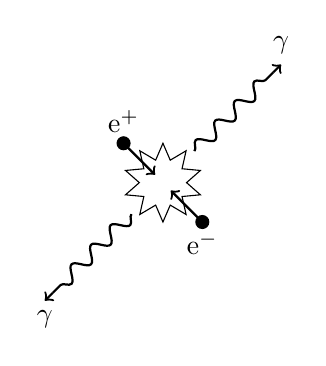
\begin{tikzpicture}[thick]
\draw[->]  (-0.5,0.5) node[anchor=south] {e$^{+}$} --(-0.1,0.1); 
\draw[->]  (0.5,-0.5) node[anchor=north] {e$^{-}$} --(0.1,-0.1);
\draw[fill=black] (0.5,-0.5) circle (0.075) ;
\draw[fill=black] (-0.5,0.5) circle (0.075) ;
\draw[decorate,decoration={snake}] (0.4,0.4)--(1.4,1.4);
\draw[->](1.4,1.4)--(1.5,1.5)node[anchor=south]{$\gamma$};
\draw[decorate,decoration={snake}] (-0.4,-0.4)--(-1.4,-1.4);
\draw[->](-1.4,-1.4)--(-1.5,-1.5)node[anchor=north]{$\gamma$};
\begin{scope}[thin]
\node [star, star points=10, star point height=.2cm, minimum size=1cm, draw]
at (0,0) {};
\end{scope}
\end{tikzpicture}

The energy they contain due to their masses is $2m_{\mathrm{e}}c^{2}$, where $m_{\mathrm{e}}$ is the rest mass of an electron.  The total energy of the two\footnote{Two photons are needed to conserve both energy and momentum.} photons produced is also $2m_{\mathrm{e}}c^{2}$, due to conservation of energy\footnote{The annihilating particles are assumed to be at rest.}, and each photons has energy $m_{\mathrm{e}}c^{2}(=hf)$.  This allows the frequency of the gamma ray photons to be identified (which give an indication of which particles annihilated).

\subsection{Pair production}

A photon of electromagnetic radiation can interact with an atomic nucleus or an electron and creates a particle-antiparticle pair.  It has to interact with a nucleus or electron to conserve both energy and momentum; the nucleus or electron recoils (consider the time-reversal of this process in the zero-momentum frame to see this):\\

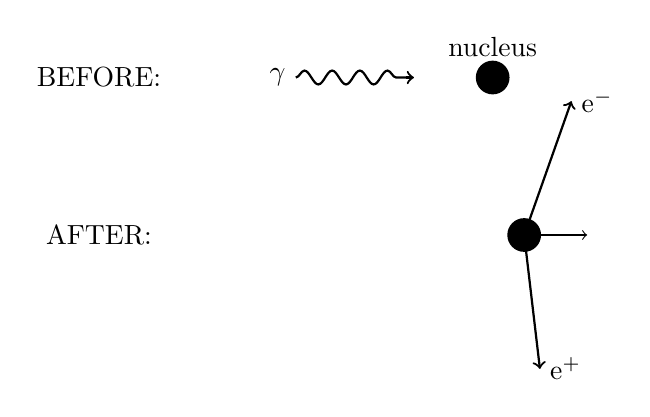
\begin{tikzpicture}[thick]
\draw (-2,0) node  {BEFORE:};
\draw (-2,-2) node {AFTER:};
\draw[fill=black] (3,0) circle (0.2) node[above=4pt]{nucleus};
\draw[decorate,decoration={snake}] (0.5,0)node[anchor=east]{$\gamma$}--(1.9,0);
\draw[->] (1.9,0)--(2.0,0);
\draw[fill=black]  (3,-2) ++(0.4,0) circle (0.2);
\begin{scope}[thin]
\draw[->](3,-2) ++(0.4,0)--++(0.8,0);
\end{scope}
\draw[->](3.4,-2) ++(0,0)--++(0.2+0.4,1.7)node[anchor=west]{e$^{-}$};
\draw[->](3.4,-2) ++(0,0)--++(-0.2+0.4,-1.7)node[anchor=west]{e$^{+}$};
\end{tikzpicture}

Commonly, electron-positron pairs are produced, as these are relatively light, and so the energy of the incoming photon does not have to be too high.

For pair production, the total mass produced is $2m_{\mathrm{e}}c^{2}$, so the minimum energy of the photon must be $E=hf=2m_{\mathrm{e}}c^{2}$.  Any excess energy of the photon goes into kinetic energy of the electron and positron.

In detectors, a magnetic field is applied, and pair production can be easily seen as the pair curve away in opposite directions due to their opposite charges.

\subsection{The photon model of electromagnetic radiation}

Light, and all of the electromagnetic spectrum, can be described as a wave, and this adequately explains effects such as diffraction and reflexion.  However, physicists found that some phenomena, such as the photoelectric effect\footnote{This will be discussed in more detail later in the module.  Briefly, it is the emission of electrons from the surface of a metal.  It is noted that (i) there is a minimum frequency of light to cause emission (the electrons need a minimum energy to escape) and (ii) the kinetic energy of the electrons emitted increases as the frequency of the light increases (photons have more energy to give to the electrons).} and the black body radiation spectrum\footnote{which you don't have to know about at A-level.}, could not be described in this way.

In 1900, Max Planck came up with a suggestion that objects which emit electromagnetic radiation do so in discrete amounts.  He said that the energy was proportional to the frequency of the radiation, i.e.
\[E\propto f,\mathrm{~or}\]
\[E=hf,\]
where $h$ is the Planck constant, 6.64\e{34}~J~s.

The individual packets, or quanta, of electromagnetic radiation are called photons.  Photons are indivisible, and when they collide with e.g. an electron, all or none of the energy is given to the electron.

\subsubsection{Examples}

\begin{enumerate}
\item Calculate the photon energy of
\begin{enumerate}
\item a gamma ray of frequency 2\e{22}~Hz\\
$E=hf=6.64\e{-34}~\mathrm{J~s~}\times 2\e{22}~\mathrm{s}^{-1}=1.33\e{-11}$~J.
\item red light of wavelength 7.8\e{-7}~m\\
$E=hf$, as $c=f\lambda$ (where $c=3\e{8}$~m~s$^{-1}$)\\
$E=\dfrac{hc}{\lambda}=\dfrac{6.64\e{-34}~\mathrm{J~s~}\times 3\e{8}~\mathrm{m~s}^{-1}}{7.8\e{-7}~\mathrm{m}}=2.55\e{-19}$~J.
\end{enumerate}
\item A sodium light emits yellow light of frequency 5.1\e{14}~Hz.  If it is a 30~W lamp, how many photons are emitted per second?\\
$30~\mathrm{W}=30$~J~s$^{-1}.$\\
$P=\dfrac{E}{t}=\mathrm{photon~number~per~unit~time}\times hf,$\\
$\mathrm{photon~number~per~unit~time}=\dfrac{P}{hf}=\dfrac{30~\mathrm{J}~\mathrm{s}^{-1}}{6.64\e{-34}~\mathrm{J~s~}\times 5.1\e{14}~\mathrm{Hz}}=8.9\e{19}~\mathrm{s}^{-1}.$
\end{enumerate}

\section{Forces between elementary particles}

There are four forces which act between elementary particles.  Gravity and the electromagnetic force are the two familiar forces, and in addition there are two nuclear forces, the strong interaction and the weak interaction.\\

\begin{tabular}{lcc}
\hline
Interaction & Range / m & Relative strength\\
\hline
Strong & $\sim 10^{-15}$ & 1\\
Electromagnetism & $\infty$ & $10^{-2}$\\
Weak & $\sim 10^{-18}$ & $\sim 10^{-7}$\\
Gravity & $\infty$ & $\sim 10^{-39}$\\
\hline
\end{tabular}\\

\subsubsection{Gravity}
Gravity affects all particles which have mass.  It has an infinite range and is purely attractive.  It governs the structure of stars, galaxies \&\ c. and its exact strength will determine the fate of the universe.

\subsubsection{Electromagnetism}
This force affects all particles with charge.  It is much stronger than gravity and also of infinite range, but it tends to cancel in bulk matter as this normally comprises nearly exactly equal numbers of positively and negatively charged particles.

\subsubsection{Strong}

The strong force is only felt by hadrons, which are all made from quarks.  The strong force is short range, and only affects nearest neighbours in the nucleus, as its range is the same as the diameter of a nucleon:\\

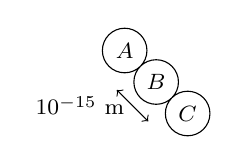
\begin{tikzpicture}
\footnotesize
\draw (-0.4,0.4) node {$A$} circle (0.283) (0,0) node {$B$} circle (0.283) (0.4,-0.4) node {$C$} circle (0.283);
\draw[<->] (-0.3,-0.3) node[anchor=east] {$10^{-15}$~m} ++(-0.2,0.2)--++(0.4,-0.4);
\end{tikzpicture}\\
i.e. $A$ and $B$ are attracted by the strong force, as are $B$ and $C$, but $A$ and $C$ are not.

The strong force is always attractive, and charge independent (the same for n--p, p--p and n--n).

\subsubsection{Weak}

When a neutron decays into a proton and an electron, and antineutrino is formed.  This is uncharged and does not feel the strong force, so another short range interaction must be involved.  The weak interaction affects both hadrons and leptons, and is usually associated with decays of various particles.  Weak decays generally take place much more slowly than strong decays (the stronger the interaction, the quicker the decay).

When {\bf strange} particles decay, they do so by the weak interaction, and strangeness is not conserved.

\subsection{Modern explanation of the four forces}

It was previously thought that a particle would create a field which exists throughout all space, and affects any particles in the field.  The modern view, however, is that two particles exert a force on one another due to the transfer of a virtual particle, which carries the force (this is known as second quantization).  These particles are called exchange particles, and are gauge bosons.

The energy to create these particles comes from the Heisenberg uncertainty principle, which allows energy $\Delta E$ to be created for a time $\Delta t$, so long as
\[\Delta E \times \Delta t < \hbar,\]
where $\hbar=\dfrac{h}{2\pi}=1.05\e{-34}$~J~s, known as the reduced Planck constant.

The energy `borrowed' creates the mass of the exchange particle, and therefore more massive exchange particles cannot exist for a long time, which puts an upper limit on how far they may travel, and thus the range of the forces produced.  This suggests:
\begin{itemize}
\item The range of electromagnetic and gravitational forces is infinite, so the exchange particles for these forces must be massless.
\item The range of the strong and weak are finite, so the exchange particles have mass, and the mass of the weak exchange particle is larger.
\end{itemize}

\subsection{The strong interaction}

Protons and neutrons are held together by the strong force (which acts on all hadrons).  As the range of the strong force is $10^{-15}$~m, and assuming the exchange particle has a speed close to that of light, it must exist for $\sim 10^{-23}$~s.  This allows the mass of the exchange particle to be calculated, and it is found that the particle is the pi-meson or pion.

It can be shown as:\\

\noindent \begin{minipage}{0.5\textwidth}
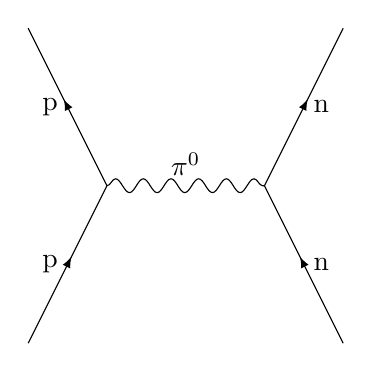
\begin{tikzpicture}
\draw[style={boson}]
  (0, 0) -- node[auto] {$\pi^{0}$} (2,0) ;
    \draw[style={electron}]
   (-1, -2) -- node[left] {p} (0, 0);
  \draw[style={electron}]
  (0, 0) -- node[left] {p} (-1, 2) ;
  \draw[style={electron}]
   (3, -2)  -- node[right] {n} (2, 0) ;
  \draw[style={electron}]
  (2, 0) -- node[right] {n} (3, 2) ;
\end{tikzpicture}
\end{minipage}
\begin{minipage}{0.5\textwidth}
The direction of the paths does not show the direction of the particles, only of the interaction.
\end{minipage}\\

At a deeper level, the quarks themselves in the hadrons are held together by gluons:\\

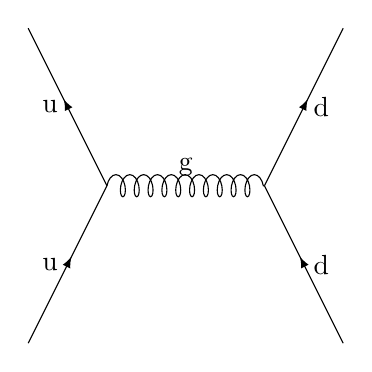
\begin{tikzpicture}
\draw[style={gluon}]
  (0, 0) -- node[auto] {g} (2,0) ;
    \draw[style={electron}]
   (-1, -2) -- node[left] {u}(0, 0);
  \draw[style={electron}]
  (0, 0) -- node[left]{u}(-1, 2) ;
  \draw[style={electron}]
   (3, -2) --node[right] {d}  (2, 0) ;
  \draw[style={electron}]
  (2, 0) -- node[right] {d} (3, 2) ;
\end{tikzpicture}\\

The pion can be seen to exist to carry the gluons between the hadrons.

\subsection{The weak interaction}

The weak interaction is very short range which suggests the exchange particle is massive.  On of the characteristics of the weak force is that it is responsible for decays of particles.  The weak force causes a change in the quark structure of a hadron.

There are three particles which can carry the weak force, $mathrm{W}^{+}$, $\mathrm{W}^{-}$ and $\mathrm{Z}^{0}$, and these act on leptons and hardrons.

The most common weak interaction is beta decay.  In this, a neutron decays into a proton, and into an electron and anti-electron neutrino through the weak interaction:
\[\mathrm{n}\longrightarrow\mathrm{p}+\mathrm{e}^{-}+\bar{\nu}_\mathrm{e},\]
which is shown as:\\

\noindent \begin{minipage}{0.5\textwidth}
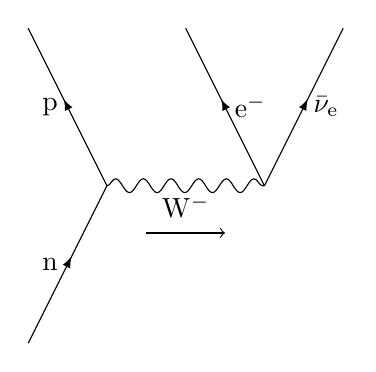
\begin{tikzpicture}
\draw[style={boson}]
  (0, 0) -- node[below] {$\mathrm{W}^{-}$} (2,0) ;
   \draw[->] (0.5,-0.6)--(1.5,-0.6);
    \draw[style={electron}]
   (-1, -2) -- node[left] {n}(0, 0);
   
  \draw[style={electron}]
  (0, 0) -- node[left] {p}(-1, 2) ;
  \draw[style={electron}]
   (2, 0)  -- node[right] {e$^{-}$}(1, 2) ;
  \draw[style={electron}]
  (2, 0) -- node[right] {$\bar{\nu}_{\mathrm{e}}$}(3, 2) ;
\end{tikzpicture}  
\end{minipage}
\begin{minipage}{0.5\textwidth}
The W$^{-}$ is the carrier of the weak force.  It needs to be negative to conserve charge.
\end{minipage}

The weak force is the only force which acts on neutrinos (other than gravity), and this is why they are weakly interacting.

Weak force is responsible for the changing of a strange quark into a non-strange quark, and this is why strangeness is changed in a weak decay.

\subsection{Electromagnetism}

The electromagnetic force is exerted between any charged particles, and is described by the theory known as {\bf quantum electrodynamics (QED)}.  As the range of the force is infinite, the exchange particle is massless, and is a virtual photon.

e.g. electron--electron scattering:

\begin{tikzpicture}
\draw[style={boson}]
  (0, 0) -- node[auto] {$\gamma$} (2,0) ;
    \draw[style={electron}]
   (-1, -2) -- node[left] {e$^{-}$}(0, 0);
  \draw[style={electron}]
  (0, 0) -- node[left] {e$^{-}$}(-1, 2) ;
  \draw[style={electron}]
   (3, -2)  -- node[right] {e$^{-}$}(2, 0) ;
  \draw[style={electron}]
  (2, 0) -- node[right] {e$^{-}$}(3, 2) ;
\end{tikzpicture}

\subsection{Gravity}
The particle responsible for the gravitational interaction is postulated to be the graviton.  It ought to have zero mass and zero charge, but has not yet been detected.

\subsection{Unification}
It is believed that all four forces can be theoretically united, to show that they are all different aspects of one force.  There has been some success already, namely the unification of the electromagnetic with the weak interactions, and it is an aim of modern physics to unite the others in a unified theory (sometimes known as a `grand unified theory' or `theory of everything'\ldots\ )


\section{Classification of particles}
All fundamental particles fall into one of three families: the leptons, the quarks, and the gauge bosons.

\subsection{Leptons}

There are twelve different leptons, which do not experience the strong interaction (and uncharged leptons do not feel the electromagnetic force either).  They are the electron, the muon and the tau, each has an associated neutrino, and they all have antiparticles.  The standard model, a collection of related gauge theories currently used in particle physics, suggests that these are the only leptons which exist.  The electron and positron are stable.

The muon ($\mu^{-}$) was discovered in cosmic rays in 1937, and has the same charge as the electron, but is 207 times heavier.  The neutrino which accompanies its reactions was found to be different from the neutrino in electron reactions in 1962.

The tau ($\tau^{-}$) was discovered in 1978, and is also the same charge as the electron, but is around 3500 times more massive.  The neutrino that accompanies the tau was only discovered in 2000, though its existence was assumed in the standard model long before this (leaving the Higgs boson as the last particle in the standard model yet to be observed).

Both the muon and the tau decay into electrons.

To help identify which reactions may take place, all particles are assigned a series of numbers:\\

\begin{tabular}{lccccc}
\hline
\hline
Name & Symbol & Charge ($Q$) / $e$ & \multicolumn{3}{c}{Lepton numbers}\\
&&&$L_{\mathrm{e}}$&$L_{\mu}$&$L_{\tau}$\\
\cline{4-6}
\hline
electron & $\mathrm{e}^{-}$ & $-1$ & $1$ & $0$ & $0$\\
positron & $\mathrm{e}^{+}$ & $+1$ & $-1$ & $0$ & $0$\\
electron neutrino & $\nu_{\mathrm{e}}$ & $0$ & $1$ & $0$ & $0$\\
antielectron neutrino & $\bar{\nu}_{\mathrm{e}}$ & $0$ & $-1$ & $0$ & $0$\\
\hline
muon & $\mu^{-}$ & $-1$ & $0$ & $1$ & $0$\\
antimuon & $\mu^{+}$ & $+1$ & $0$ & $-1$ & $0$\\
muon neutrino & $\nu_{\mu}$ & $0$ & $0$ & $1$ & $0$\\
antimuon neutrino & $\bar{\nu}_{\mu}$ & $0$ & $0$ & $-1$ & $0$\\
\hline
tau & $\tau^{-}$ & $-1$ & $0$ & $0$ & $1$\\
antitau & $\tau^{+}$ & $+1$ & $0$ & $0$ & $-1$\\
tau neutrino & $\nu_{\tau}$ & $0$ & $0$ & $0$ & $1$\\
antitau neutrino & $\bar{\nu}_{\tau}$ & $0$ & $0$ & $0$ & $-1$\\
\hline
\hline
\end{tabular}

\paragraph{Notes}\begin{enumerate}
\item Baryon number $B$ and strangeness $S$ are zero for all leptons.
\item Only leptons have lepton numbers, and lepton number must be conserved (remain unchanged) in all particle interactions or decays.
\end{enumerate}

\subsection{Quarks}
Although quarks are fundamental particles, they NEVER exist in isolation, as single, free quarks.  The standard model suggests there should be six `flavours' of quark (i.e. six quarks and six antiquarks, which match the twelve leptons).  These all experience all of the four forces, and always combine to form heavier particles called hadrons.

\newpage

The six quarks are:\\

\noindent\begin{tabular}{lccc}
\hline
\hline
Quark & Symbol & Charge ($Q$) / $e$ & mass / $m_{\mathrm{p}}$\\
\hline
up & u & $+\frac{2}{3}$ & 0.33\\
antiup & $\bar{\mathrm{u}}$ & $-\frac{2}{3}$ & 0.33\\ 
down & d & $-\frac{1}{3}$ & 0.34\\
antidown & $\bar{\mathrm{d}}$ & $+\frac{1}{3}$ & 0.34\\
\hline
charm & c & $+\frac{2}{3}$ & 1.59\\
anticharm & $\bar{\mathrm{c}}$ & $-\frac{2}{3}$ & 1.59\\
strange & s & $-\frac{1}{3}$ & 0.53\\
antistrange & $\bar{\mathrm{s}}$ & $+\frac{1}{3}$ & 0.53\\
\hline
top & b & $+\frac{2}{3}$ & 185.5\\
antitop & $\bar{\mathrm{b}}$ & $-\frac{2}{3}$ & 185.5\\
bottom & t & $-\frac{1}{3}$ & 4.80\\
antibottom & $\bar{\mathrm{t}}$ & $+\frac{1}{3}$ & 4.80\\
\hline
\hline
\end{tabular}\\

We shall only consider combinations of up, down and strange quarks (and their antiquarks), although the other quarks follow the same patterns.  However, it is more difficult to make the heavier quarks as much more energy is required.

The particles that quarks make up (called hadrons) fall into two categories:

\subsubsection{Baryons ($\mathrm{q}\mathrm{q}\mathrm{q})$ or $\bar{\mathrm{q}}\bar{\mathrm{q}}\bar{\mathrm{q}}$)}

Baryons have a baryon number $B$ of $+1$, are made of three quarks, and have a lepton number $L$ of $0$.  They may or may not have a strangeness, which depends on whether they contain strange quarks. (Antibaryons contain three antiquarks, and have a baryon number of $-1$.)

There are many more baryons than the combinations of the six quark flavours suggests ($^{6}C_{3}\times 2=40$), as the quarks have energy levels (like electrons).  The $\Delta^{+}$ (delta plus) particle, for example, has the same quark structure as the proton, but is more massive as its quarks have more energy, and spin differently.

Of all the baryons, only the proton is stable (and the standard model suggests its half life may be around $10^{32}$~years, cf. present age of the universe $\sim 10^{10}$~years).

\begin{tabular}{lcccc}
\hline
\hline
Name & Symbol & Charge ($Q$) & Baryon No. ($B$) & Strangeness ($S$)\\
\hline
proton & p & $+1$ & $1$ & $0$ \\
antiproton & $\bar{\mathrm{p}}$ & $-1$ & $-1$ & $0$ \\
neutron & n & $0$ & $1$ & $0$ \\
antineutron & $\bar{\mathrm{n}}$ & $0$ & $-1$ & $0$ \\
lambda & $\bar{\Lambda}^{0}$ & $0$ & $1$ & $-1$ \\
antilambda & $\bar{\Lambda}^{0}$ & $0$ & $-1$ & $+1$ \\
sigma plus & $\bar{\Sigma}^{+}$ & $+1$ & $1$ & $-1$ \\
antisigma plus & $\bar{\Sigma}^{+}$ & $-1$ & $-1$ & $+1$ \\
sigma zero & $\bar{\Sigma}^{0}$ & $0$ & $1$ & $-1$ \\
antisigma zero & $\bar{\Sigma}^{0}$ & $0$ & $-1$ & $+1$ \\
sigma minus & $\bar{\Sigma}^{-}$ & $-1$ & $1$ & $-1$ \\
antisigma minus & $\bar{\Sigma}^{-}$ & $+1$ & $-1$ & $+1$ \\
xi minus & $\bar{\Xi}^{-}$ & $-1$ & $1$ & $-2$ \\
antixi minus & $\bar{\Xi}^{-}$ & $+1$ & $-1$ & $+2$ \\
xi zero & $\bar{\Xi}^{0}$ & $0$ & $1$ & $-2$ \\
antixi zero & $\bar{\Xi}^{0}$ & $0$ & $-1$ & $+2$ \\
omega & $\bar{\Omega}^{-}$ & $-1$ & $1$ & $-3$ \\
antiomega & $\bar{\Omega}^{-}$ & $+1$ & $-1$ & $+3$ \\
\hline
\hline
\end{tabular}

\subsubsection{Mesons $\mathrm{q}\bar{\mathrm{q}}$}

Mesons have a baryon number of zero, and a lepton number of zero.  They are made up of a quark and an antiquark.  None of the mesons are stable.

When a meson is made of a quark-antiquark pair (e.g. $\mathrm{u}\bar{\mathrm{u}}$) these quarks do not annihilate, as they have another property (colour\footnote{Colour is just a label -- not a real colour! -- for the charge of the strong interaction.  Unlike electric charge ($+$ or $-$), the strong charge comes in three colours: R, G and B.}) which is different for the two quarks.\\

\begin{tabular}{lcccc}
\hline
\hline
Name & Symbol & Charge ($Q$) & Baryon No. ($B$) & Strangeness ($S$)\\
\hline
{\bf Pions} \\
pi-zero & $\pi^{0}$ & $0$ & $0$ & $0$ \\
antipi-zero & $\pi^{0}$ & $0$ & $0$ & $0$ \\
pi-plus & $\pi^{+}$ & $+1$ & $0$ & $0$ \\
pi-minus* & $\pi^{-}$ & $-1$ & $0$ & $0$ \\
\hline
{\bf Kaons} \\
K-zero & $\mathrm{K}^{0}$ & $0$ & $0$ & $1$ \\
antiK-zero & $\bar{\mathrm{K}}^{0}$ & $0$ & $0$ & $-1$ \\
K-plus & $\mathrm{K}^{+}$ & $+1$ & $0$ & $1$ \\
K-minus* & $\mathrm{K}^{-}$ & $-1$ & $0$ & $-1$ \\
\hline
\hline
\end{tabular}
*Due to their composition, the antiparticles of the pi-plus and the K-plus are not the antipi-plus and K-plus (as might be expected), but are instead the pi-minus and K-minus.

There are many more mesons than those listed!

%\subsection{Guage Bosons}

\section{Quark structure of hadrons}

In the early 1960s, the number of known hadrons was large enough for physicists to start to make patterns and reduce the large numbers to a simpler scheme.  Murray Gell-Mann and George Zweig put together the theory that the hadrons were made up of smaller constituents named quarks.

It was initially thought that there were only three flavours of quark, up, down and strange.  Current theory suggests there are six.  The properties of the first three quarks to be discovered are as follows (lepton numbers are all zero):

\noindent\begin{tabular}{lccc}
\hline
\hline
Quark & Charge ($Q$) / $e$ & Baryon number ($B$) & Strangeness ($S$) \\
\hline
up (u) & $+\frac{2}{3}$ & $+\frac{1}{3}$ & $0$ \\
antiup ($\bar{\mathrm{u}}$) & $-\frac{2}{3}$ & $-\frac{1}{3}$ & $0$ \\ 
down (d) & $-\frac{1}{3}$ & $+\frac{1}{3}$ & $0$ \\
antidown ($\bar{\mathrm{d}}$) & $+\frac{1}{3}$ & $-\frac{1}{3}$ & $0$ \\
strange (s) & $-\frac{1}{3}$ & $+\frac{1}{3}$ & $-1$ \\
antistrange ($\bar{\mathrm{s}}$) & $+\frac{1}{3}$ & $-\frac{1}{3}$ & $+1$ \\
\hline
\hline
\end{tabular}

\subsection{Quark combinations}

\begin{enumerate}
\item Baryons are composed of three quarks ($\mathrm{q}\mathrm{q}\mathrm{q})$) and antibaryons are composed of three antiquarks ($\bar{\mathrm{q}}\bar{\mathrm{q}}\bar{\mathrm{q}}$).
\item Mesons are composed of a quark and an antiquark ($\mathrm{q}\bar{\mathrm{q}}$).
\end{enumerate}

The actual quarks involved in a particular particle can be calculated from the quantum numbers of that particle, although the proton and neutron should be known.\\

\begin{tabular}{lclc}
\hline
\hline
Particle & Quark content & Antiparticle & Quark content \\
\hline
p & $\mathrm{u}\mathrm{u}\mathrm{d}$ & $\bar{\mathrm{p}}$ & $\bar{\mathrm{u}}\bar{\mathrm{u}}\bar{\mathrm{d}}$ \\
n & $\mathrm{u}\mathrm{d}\mathrm{d}$ & $\bar{\mathrm{n}}$ & $\bar{\mathrm{u}}\bar{\mathrm{d}}\bar{\mathrm{d}}$ \\
$\pi^{+}$ & $\mathrm{u}\bar{\mathrm{d}}$ & $\pi^{-}$ & $\bar{\mathrm{u}}\mathrm{d}$ \\
$\pi^{0}$ & $\mathrm{u}\bar{\mathrm{u}},\mathrm{d}\bar{\mathrm{d}}$ & $\pi^{0}$ & $\mathrm{u}\bar{\mathrm{u}},\mathrm{d}\bar{\mathrm{d}}$ \\
$\mathrm{K}^{-}$ & $\mathrm{u}\bar{\mathrm{s}}$ & $\mathrm{K}^{-}$ & $\bar{\mathrm{u}}\mathrm{s}$ \\
$\mathrm{K}^{0}$ & $\mathrm{d}\bar{\mathrm{s}}$ & $\bar{\mathrm{K}}^{0}$ & $\bar{\mathrm{d}}\mathrm{s}$ \\
\hline
\hline
\end{tabular}

The $\pi^{0}$ is actually a combination of $\mathrm{u}\bar{\mathrm{u}}+\mathrm{d}\bar{\mathrm{d}}$, but can be regarded as just one of these.  Although the u and $\bar{\mathrm{u}}$ appear to be antiparticles, there are three `colours' of quarks, so the u and $\bar{\mathrm{u}}$ in a $\pi^{0}$, having different colours, do not annihilate.

Experimental evidence for quarks was first provided in 1969 when electrons of de Broglie wavelength $10{-16}$~m were fired at protons.  As this is about 10 times smaller than the proton, these electrons can resolve internal structure, finding three particles inside the proton.

\section{Particle Interactions}

An interaction describes a collision between two particles producing others, or a decay of an unstable particle.  In every interaction:
\begin{enumerate}
\item mass/energy must be conserved
\item momentum must be conserved
\item charge $Q$ must be conserved
\item baryon  number $B$ must be conserved
\item lepton number $L$ must be conserved
\item strangeness $S$ \begin{enumerate}\item is conserved in collisions
\item changes by $\pm 1$ in a weak decay\end{enumerate}
\end{enumerate}

\paragraph{Notes}
\begin{itemize}
\item Strange particles decay by strong or weak decays (the typical lifetimes for strong decays are typically $10^{-23}$~s, and weak decays typically $10^{-8}$~s).  We shall presume all strange decays to be weak, i.e.\ strangeness will change if a strange particle decays, as a strange quark changes into a non-strange quark.
\item Energy/mass considerations will not be taken into account, as in principle any energy can be converted into mass in accelerators.
\end{itemize}

The general method of solution is to write $Q$, $B$, $L$, $S$ below the interaction and check for conservation.

\subsubsection{Examples}

\begin{enumerate}
\item Which of the following are possible?\begin{enumerate}
\item \begin{tabular}[t]{lccccccc}
& $\mathrm{n}$ & $\longrightarrow$ & $\mathrm{p}$ & $+$ & $\mathrm{e}^{-}$ & $+$ & $\bar{\nu}_{e}$\\
$Q$ & $0$ & $\rightarrow$ & $+1$ & & $-1$ & & $0$ \\
$B$ & $+1$ & $\rightarrow$ & $+1$ & & $0$ & & $0$ \\
$L$ & $0$ & $\rightarrow$ & $0$ & & $+1$ & & $-1$ \\
$S$ & $0$ & $\rightarrow$ & $0$ & & $0$ & & $0$ \\
\end{tabular}\\
All of the quantities are conserved, so this $\beta$ decay is possible.
\item \begin{tabular}[t]{lccccc}
& $\Lambda^{0}$ & $\longrightarrow$ & $\mathrm{p}$ & $+$ & $\pi^{-}$ \\
$Q$ & $0$ & $\rightarrow$ & $+1$ & & $-1$ \\
$B$ & $+1$ & $\rightarrow$ & $+1$ & & $0$  \\
$L$ & $0$ & $\rightarrow$ & $0$ & & $0$  \\
$S$ & $-1$ & $\rightarrow$ & $0$ & & $0$ \\
\end{tabular}\\
$Q$, $B$ and $L$ are conserved, and the strangeness changes by $+1$ in this weak decay.
\end{enumerate}
\item Identify particle X:\\
\begin{tabular}[t]{lccccccccccc}
& $\mathrm{p}$ & $+$ & $\pi^{-}$ & $\longrightarrow$ & $\mathrm{n}$ & $+$ & $\pi^{0}$ & $+$ & $\pi_{-}$ & $+$ & X\\
$Q$ & $+1$ & & $-1$ & $\rightarrow$ & $0$ & & $0$ & & $-1$ & & $+1$ \\
$B$ & $+1$ & & $0$ & $\rightarrow$ & $+1$ & & $0$ & & $0$ & & $0$ \\
$L$ & $0$ & & $0$ & $\rightarrow$ & $0$ & & $0$ & & $0$ & & $0$ \\
$S$ & $0$ & & $0$ & $\rightarrow$ & $0$ & & $0$ & & $0$ & & $0$ \\
\end{tabular}\\
From its properties, the particle X must be a $\pi^{+}$.
\end{enumerate}


\section{Feynman diagrams}
Feynman diagrams represent particle interactions -- the angles between the particle lines are not significant, only the sequence of events.  The force is shown via an exchange particle.

\subsection{$\beta^{-}$ decay}
A neutron decays into a proton (a down quark changes into an up quark), emitting a beta particle and an antielectron neutrino:
\[\mathrm{n}\longrightarrow\mathrm{p}+\mathrm{e}^{-}+\bar{\nu}_{\mathrm{e}}\]

\noindent \begin{minipage}{0.4\textwidth}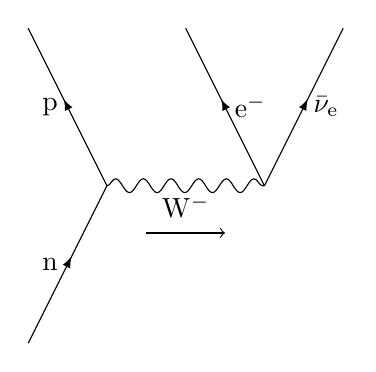
\begin{tikzpicture}
\draw[style={boson}]
  (0, 0) -- node[below] {$\mathrm{W}^{-}$} (2,0) ;
   \draw[->] (0.5,-0.6)--(1.5,-0.6);
    \draw[style={electron}]
   (-1, -2) -- node[left] {n}(0, 0);
  \draw[style={electron}]
  (0, 0) -- node[left] {p}(-1, 2) ;
  \draw[style={electron}]
   (2, 0)  -- node[right] {e$^{-}$}(1, 2) ;
  \draw[style={electron}]
  (2, 0) -- node[right] {$\bar{\nu}_{\mathrm{e}}$}(3, 2) ;
\end{tikzpicture} \end{minipage}\begin{minipage}[c]{0.1\textwidth}OR\end{minipage}
\begin{minipage}{0.4\textwidth}
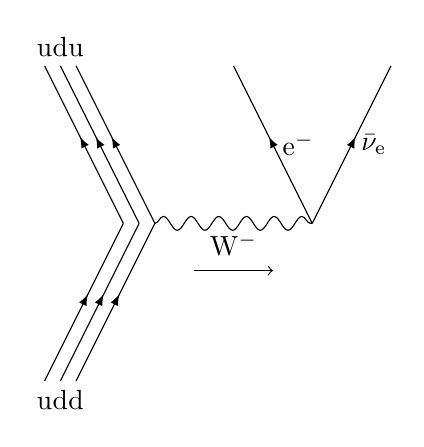
\begin{tikzpicture}
\draw[style={boson}]
  (0, 0) -- node[below] {$\mathrm{W}^{-}$} (2,0) ;
   \draw[->] (0.5,-0.6)--(1.5,-0.6);
    \draw[style={electron}]
   (-1, -2) node[below] {d}-- (0, 0);
  \draw[style={electron}]
  (0, 0)  -- (-1, 2) node[above] {u};
  \draw[style={electron}]
   (-1.2, -2) node[below] {d}-- (-0.2, 0);
  \draw[style={electron}]
  (-0.2, 0)  -- (-1.2, 2) node[above] {d};
  \draw[style={electron}]
   (-1.4, -2) node[below=2.5pt] {u}-- (-0.4, 0);
  \draw[style={electron}]
  (-0.4, 0)  -- (-1.4, 2) node[above] {u};
  \draw[style={electron}]
   (2, 0)  -- node[right] {e$^{-}$}(1, 2) ;
  \draw[style={electron}]
  (2, 0) -- node[right] {$\bar{\nu}_{\mathrm{e}}$}(3, 2) ;
\end{tikzpicture}  
\end{minipage}

\subsection{$\beta^{+}$ decay}
A proton decays into a neutron, emitting a neutrino and positron:
\[\mathrm{p}\longrightarrow\mathrm{n}+\mathrm{e}^{+}+\nu_{\mathrm{e}}\]

\noindent \begin{minipage}{0.4\textwidth}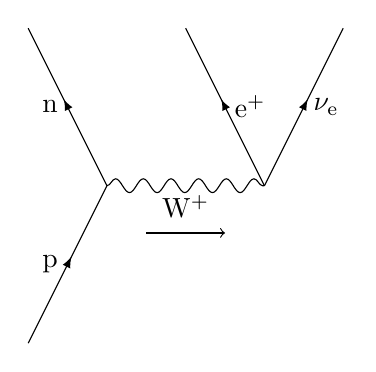
\begin{tikzpicture}
\draw[style={boson}]
  (0, 0) -- node[below] {$\mathrm{W}^{+}$} (2,0) ;
   \draw[->] (0.5,-0.6)--(1.5,-0.6);
    \draw[style={electron}]
   (-1, -2) -- node[left] {p}(0, 0);
  \draw[style={electron}]
  (0, 0) -- node[left] {n}(-1, 2) ;
  \draw[style={electron}]
   (2, 0)  -- node[right] {e$^{+}$}(1, 2) ;
  \draw[style={electron}]
  (2, 0) -- node[right] {$\nu_{\mathrm{e}}$}(3, 2) ;
\end{tikzpicture} \end{minipage}\begin{minipage}[c]{0.1\textwidth}OR\end{minipage}
\begin{minipage}{0.4\textwidth}
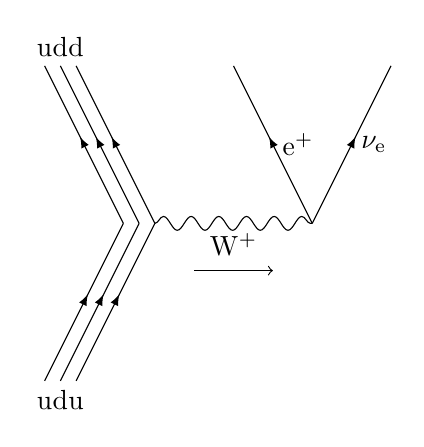
\begin{tikzpicture}
\draw[style={boson}]
  (0, 0) -- node[below] {$\mathrm{W}^{+}$} (2,0) ;
   \draw[->] (0.5,-0.6)--(1.5,-0.6);
    \draw[style={electron}]
   (-1, -2) node[below=2.5pt] {u}-- (0, 0);
  \draw[style={electron}]
  (0, 0)  -- (-1, 2) node[above] {d};
  \draw[style={electron}]
   (-1.2, -2) node[below] {d}-- (-0.2, 0);
  \draw[style={electron}]
  (-0.2, 0)  -- (-1.2, 2) node[above] {d};
  \draw[style={electron}]
   (-1.4, -2) node[below=2.5pt] {u}-- (-0.4, 0);
  \draw[style={electron}]
  (-0.4, 0)  -- (-1.4, 2) node[above] {u};
  \draw[style={electron}]
   (2, 0)  -- node[right] {e$^{+}$}(1, 2) ;
  \draw[style={electron}]
  (2, 0) -- node[right] {$\nu_{\mathrm{e}}$}(3, 2) ;
\end{tikzpicture}  
\end{minipage}


\subsection{Electron capture}

An orbiting electron can be absorbed by a proton in the nucleus:
\[\mathrm{p}+\mathrm{e}^{-}\longrightarrow\mathrm{n}+\nu_{\mathrm{e}}\]

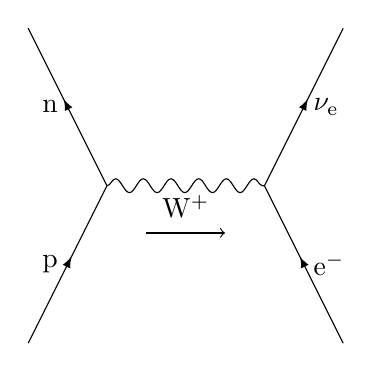
\begin{tikzpicture}
\draw[style={boson}]
 (0, 0) -- node[below] {$\mathrm{W}^{+}$} (2,0) ;
   \draw[->] (0.5,-0.6)--(1.5,-0.6);
      \draw[style={electron}]
   (-1, -2) -- node[left] {p} (0, 0);
  \draw[style={electron}]
  (0, 0) -- node[left] {n} (-1, 2) ;
  \draw[style={electron}]
   (3, -2)  -- node[right] {$\mathrm{e}^{-}$} (2, 0) ;
  \draw[style={electron}]
  (2, 0) -- node[right] {$\nu_{\mathrm{e}}$} (3, 2) ;
\end{tikzpicture}


\subsection{Neutrino--neutron collisions}
A neutron can absorb a neutrino, turning into a proton and electron:
\[\mathrm{n}+\nu_{\mathrm{e}}\longrightarrow\mathrm{p}+\mathrm{e}^{-}\]

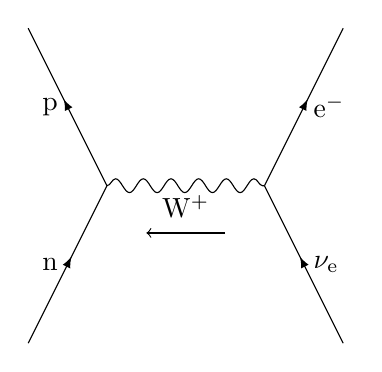
\begin{tikzpicture}
\draw[style={boson}]
 (0, 0) -- node[below] {$\mathrm{W}^{+}$} (2,0) ;
   \draw[->] (1.5,-0.6)--(0.5,-0.6);
      \draw[style={electron}]
   (-1, -2) -- node[left] {n} (0, 0);
  \draw[style={electron}]
  (0, 0) -- node[left] {p} (-1, 2) ;
  \draw[style={electron}]
   (3, -2)  -- node[right] {$\nu_{\mathrm{e}}$} (2, 0) ;
  \draw[style={electron}]
  (2, 0) -- node[right] {$\mathrm{e}^{-}$} (3, 2) ;
\end{tikzpicture}

\subsection{Antineutrino--proton collisions}
A proton can absorb an electron neutrino, becoming a neutron and emitting a positron:
\[\mathrm{p}+\nu_{\mathrm{e}}\longrightarrow\mathrm{n}+\mathrm{e}^{+}\]

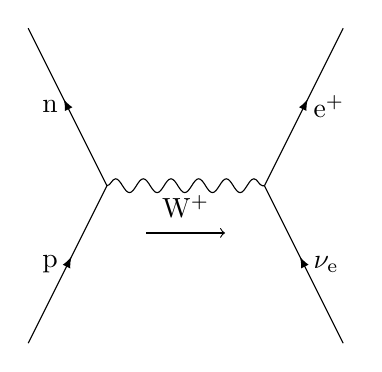
\begin{tikzpicture}
\draw[style={boson}]
 (0, 0) -- node[below] {$\mathrm{W}^{+}$} (2,0) ;
   \draw[->] (0.5,-0.6)--(1.5,-0.6);
      \draw[style={electron}]
   (-1, -2) -- node[left] {p} (0, 0);
  \draw[style={electron}]
  (0, 0) -- node[left] {n} (-1, 2) ;
  \draw[style={electron}]
   (3, -2)  -- node[right] {$\nu_{\mathrm{e}}$} (2, 0) ;
  \draw[style={electron}]
  (2, 0) -- node[right] {$\mathrm{e}^{+}$} (3, 2) ;
\end{tikzpicture}

\subsection{Electron--proton collisions}

An electron can collide with a proton, emitting a neutron and a neutrino:
\[\mathrm{p}+\mathrm{e}^{-}\longrightarrow\mathrm{n}+\nu_{\mathrm{e}}\]

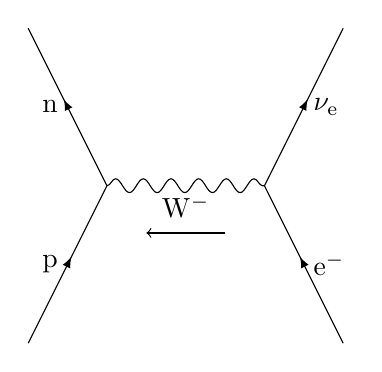
\begin{tikzpicture}
\draw[style={boson}]
 (0, 0) -- node[below] {$\mathrm{W}^{-}$} (2,0) ;
   \draw[->] (1.5,-0.6)--(0.5,-0.6);
      \draw[style={electron}]
   (-1, -2) -- node[left] {p} (0, 0);
  \draw[style={electron}]
  (0, 0) -- node[left] {n} (-1, 2) ;
  \draw[style={electron}]
   (3, -2)  -- node[right] {$\mathrm{e}^{-}$} (2, 0) ;
  \draw[style={electron}]
  (2, 0) -- node[right] {$\nu_{\mathrm{e}}$} (3, 2) ;
\end{tikzpicture}\\

All of the above interactions involve the weak interaction, and they have all been experimentally observed.
%\part{Electromagnetic radiation and quantum phenomena}




%\section{Current Electricity}

\end{document}
